\documentclass[titlepage]{article}
\usepackage{school-style-packages}
\usepackage[cc]{titlepic}

\begin{document}
\title{Developer's Guide for PINSPEC}
\titlepic{
\includegraphics[width=\textwidth]{images/pinspec.png}}
\maketitle

\section{Introduction}
\subsection{Intro to Developer's Guide}
This document is meant to provide information in addition to the user guide hosted on \href{https://github.com/mit-crpg/PINSPEC/wiki}{GitHub's wiki pages}. A number of instructions on how to install the required packages and PINSPEC, how to set up the python input files, and how to run the code can be found on the above link. Some of these info may be repeated in this document, but as a general rule of thumb users should refer to the wiki page for instructions related to using PINSPEC, and this document is reserved for info on developing PINSPEC. 

While the rest of this section would provide a high-level introduction of how PINSPEC source codes are constructed, the next couple of sections in this document would be devoted to:
\begin{itemize}
\item Review some essential instructions for installing PINSPEC and running PINSPEC, see Section~\ref{install}. 
\item Discuss how to manipulate the python codes, see Section~\ref{python}.
\item Discuss how to manipulate the C++ codes, see Section~\ref{C++}. 
\end{itemize}
Keep in mind that the above info is in addition to the commenting in the source codes and Doxygen-generated files as hosted here: \href{http://mit-crpg.github.io/PINSPEC/index.html}{Doxygen generated documents}. 


\clearpage
\subsection{Python to SWIG to C++}
Fig.~\ref{high-level} illustrates the three major components of PINSPEC: the python codes, the SWIG interface, and the C++ source codes. 

Simplified Wrapper and Interface Generator (SWIG) is open source software used in PINSPEC to wrap C++ functions for use with python. More generally, SWIG can be used to connect C/C++ with scripting languages such as Lua, Perl, PHP, Python, R, Ruby, Tcl and even non-scripting languages like C\#, Java, JavaScript, Go, Modula-3, Ocaml, Octave, and Scheme\footnote{Reference: \href{http://en.wikipedia.org/wiki/SWIG}{SWIG's wiki page}, \href{http://www.swig.org/exec.html}{SWIG's homepage}.}. 

More specifically, here is the flow of a typical simulation:
\begin{itemize}
\item Users inputs data in a python file;
\item PINSPEC python source codes process input data, perform Doppler Broadening of the cross sections if requested;
\item SWIG registers the data in C++ classes;
\item C++ contains the actualy Monte Carlo kernel, and neutrons are simulated here;
\item If any plotting is requested, generated results would be passed from C++ back to python using SWIG again and python would generate plots. 
\end{itemize}

\begin{figure}[h]
  \centering
  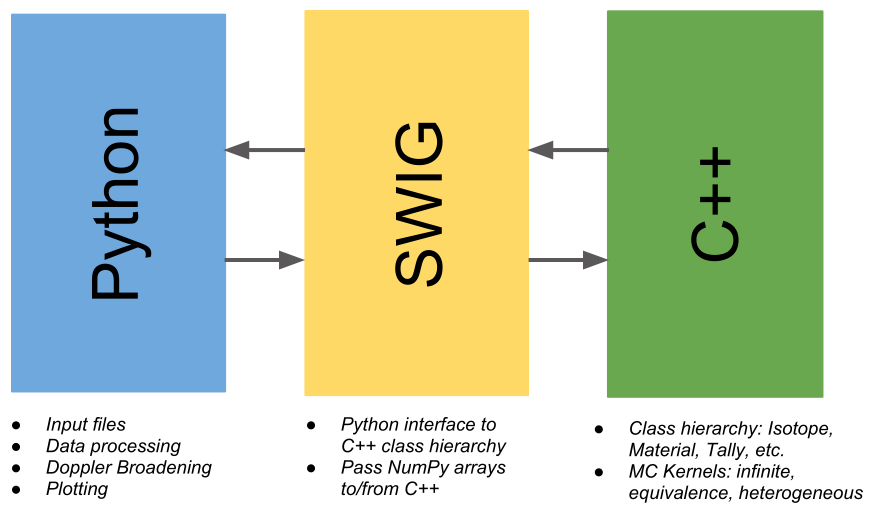
\includegraphics[width=5in]{images/high-level.png}
  \caption{Python Interfacing C++ Through SWIG} \label{high-level}
\end{figure}


\clearpage
\subsection{Major C++ Classes}
C++ using the following major classes: 
\begin{itemize}
\item Geometry: the umbrella class that knows the \# neutrons per batch, \# batches, \# threads, the type of geometry (infinite, infinite equivalent, or heterogeneous) etc. 
\item Region: a region object knows its name, material type, region type, volume and buckling. More specifically, we support 6 types of regions: 
  \begin{itemize}
    \item Infinite medium: this region covers an infinite space. 
    \item Equivalent fuel: this region is a fuel region using the infinite equivalence model. 
    \item Equivalent moderator: this region is a moderator region using the infinite equivalence model. 
    \item Bounded fuel: this region is a fuel region using the true heterogeneous model. 
    \item Bounded moderator: this region is a moderator region using the true heterogeneous model. 
    \item Bounded general: this region is a generalized region bounded by surfaces and is used in the true heterogeneous model. 
  \end{itemize}

\item Surface: Surface objects are used to bound a region. For instance, a surface object knows its name, ID \#, its surface type (x-plane, y-plane, z-cylinder), and its boundary condition (reflective, vacuum, interface). 

\item Material: an material object contains one or more isotope objects, and an material object is used to filled a region object. A material object knows basic info like its name, ID \#, material density, 


\item Isotope:

\item Neutron

\item Tally
\end{itemize}

\clearpage
\subsection{Hierarchy Diagram}
In this section we go more in depths into some of the above classes to illustrate their hierarchy. 



%%%%%%%%%%%%%%%%%%%%%%%%%%%%%%% INSTALL %%%%%%%%%%%%%%%%%%%%%%%%%%%%%%%%%
\clearpage
\section{Installation and How To Run} \label{install}
An overview of the installation procedures can be found on the users' guide. 



\clearpage
\subsection{Python 2.7 Is The Way to Go!}


\clearpage
\subsection{Additional Tools}
SSHFS: 
\begin{itemize}

\item To see what sftp subsystems are mounted: 
\begin{verbatim}
    ps aux | grep -i sftp | grep -v grep
\end{verbatim}


\end{itemize}








%%%%%%%%%%%%%%%%%%%%%%%%%%%%%%% PYTHON %%%%%%%%%%%%%%%%%%%%%%%%%%%%%%%%%
\clearpage
\section{Manipulating Python Inputs}\label{python}
\subsection{Utilizing Tally Arithmetic}
There are three tally arithmetics supported in PINSPEC: 
\begin{enumerate}
\item tally1 + tally2: creates a new tally with the correct statistics. 
\item tally1 + 3.5:
\item tally1.addFloats(numpy.array([1,2])), or addIntegers, or addDoubles. 
\end{enumerate}


\clearpage
\subsection{Example: Add A New Isotope}

\clearpage
\subsection{Example: Add A New Cross Section}






%%%%%%%%%%%%%%%%%%%%%%%%%%%%%%% C++ %%%%%%%%%%%%%%%%%%%%%%%%%%%%%%%%%
\clearpage
\section{Manipulating C++ Codes}\label{C++}
\subsection{Create A New Source File}
If you create a new source file, make sure you add it to \textit{setup.py}

\begin{itemize}
\item If you need to pass data from the python input file into the C file, or you would like to retrieve the results generated by C++ and plot or print it using python, see Section~\ref{data}. 
\item Make sure you update the doxygen commenting accordingly, and run doxygen by:
\begin{verbatim}
 doxygen docs/Doxyfile
\end{verbatim}
See more details in Section.~\ref{doxygen}. 

\item If you add in any additional functions, it is nice to update the test suites accordingly. 

\item Two examples are shown about how to add a new tally and a new surface. 
\end{itemize}

\subsection{Passing Data Between Python and C++} \label{data}
If you would like to gain access to an array of data, you need to do so through SWIG. Examples can be found in Geometry.i which contains numpy template. 


\subsection{Doxygen Commenting} \label{doxygen}
To generate html and pdf from source code commenting, run Doxygen by the following command:
\begin{verbatim}
 doxygen docs/doxygen/Doxyfile
\end{verbatim}

If you modify the source code, please update the Doxygen commenting accordingly. For instance, here are some styling suggestions:
\begin{enumerate}
\item For any class structure (including super-class and sub-class), use @class followed by class name, header file name, and header file path. Examples:
\begin{verbatim}
@class Surface Surface.h "pinspec/src/Surface.h"
@class XPlane Surface.h "pinspec/src/Surface.h"
@class YPlane Surface.h "pinspec/src/Surface.h"
\end{verbatim}
In the above examples, Surface is the super-class, and XPlane and YPlane are sub-classes. 

\item For any structure, try using @brief followed by a one-line short description, as well as @details followed by a longer description if needed. 

\item For any structure, use @param followed by parameter name and description to comment on the inputs of a method, and use @return followed by variable name and description to comment on the outputs of a method. 
\end{enumerate}


\clearpage
\subsection{Update Test Suites}

\clearpage
\subsection{Example: Implement A New Surface}

\clearpage
\subsection{Example: Implement A New Tally}


\clearpage
\subsection{Example: Implement A Monte Carlo Variance Reduction Technique}
The main kernel that performs the Monte Carlo simulation is contained in Geometry.cpp as runMonteCarloSimulation(). 

\begin{algorithm}

\caption{High Level Monte Carlo Kernel}
\begin{algorithmic}
\FOR{each batch}
\FOR{each neutron inside the batch}
\STATE Initialize neutrons:

\ENDFOR
\ENDFOR
\end{algorithmic}
\end{algorithm}

\end{document}
